\chapter{Results}
\label{cha:results}

\section{Final Distribution}
\label{sec:final-dist}

Having accounted for the systematic uncertainties, one can examine the final distribution(s). This encompasses the mass of the gaugino and smuon, where the former is part of the latter. In case of the smuon, the selected two jets and the two muons enter the invariant mass calculation. Removing the leading muon from this composition yields the gaugino case. All event selection requirements are applied and in relation to the control region BVC, only the inverted missing transverse energy requirement is reversed again $E_{\text{T}}^{\text{miss}} < 50$. Figure~\ref{fig:final-dist} shows both distributions including the data-driven background estimate.

\begin{figure}[htb!]
  \centering
  \begin{subfigure}[b]{0.495\textwidth}
    \centering
    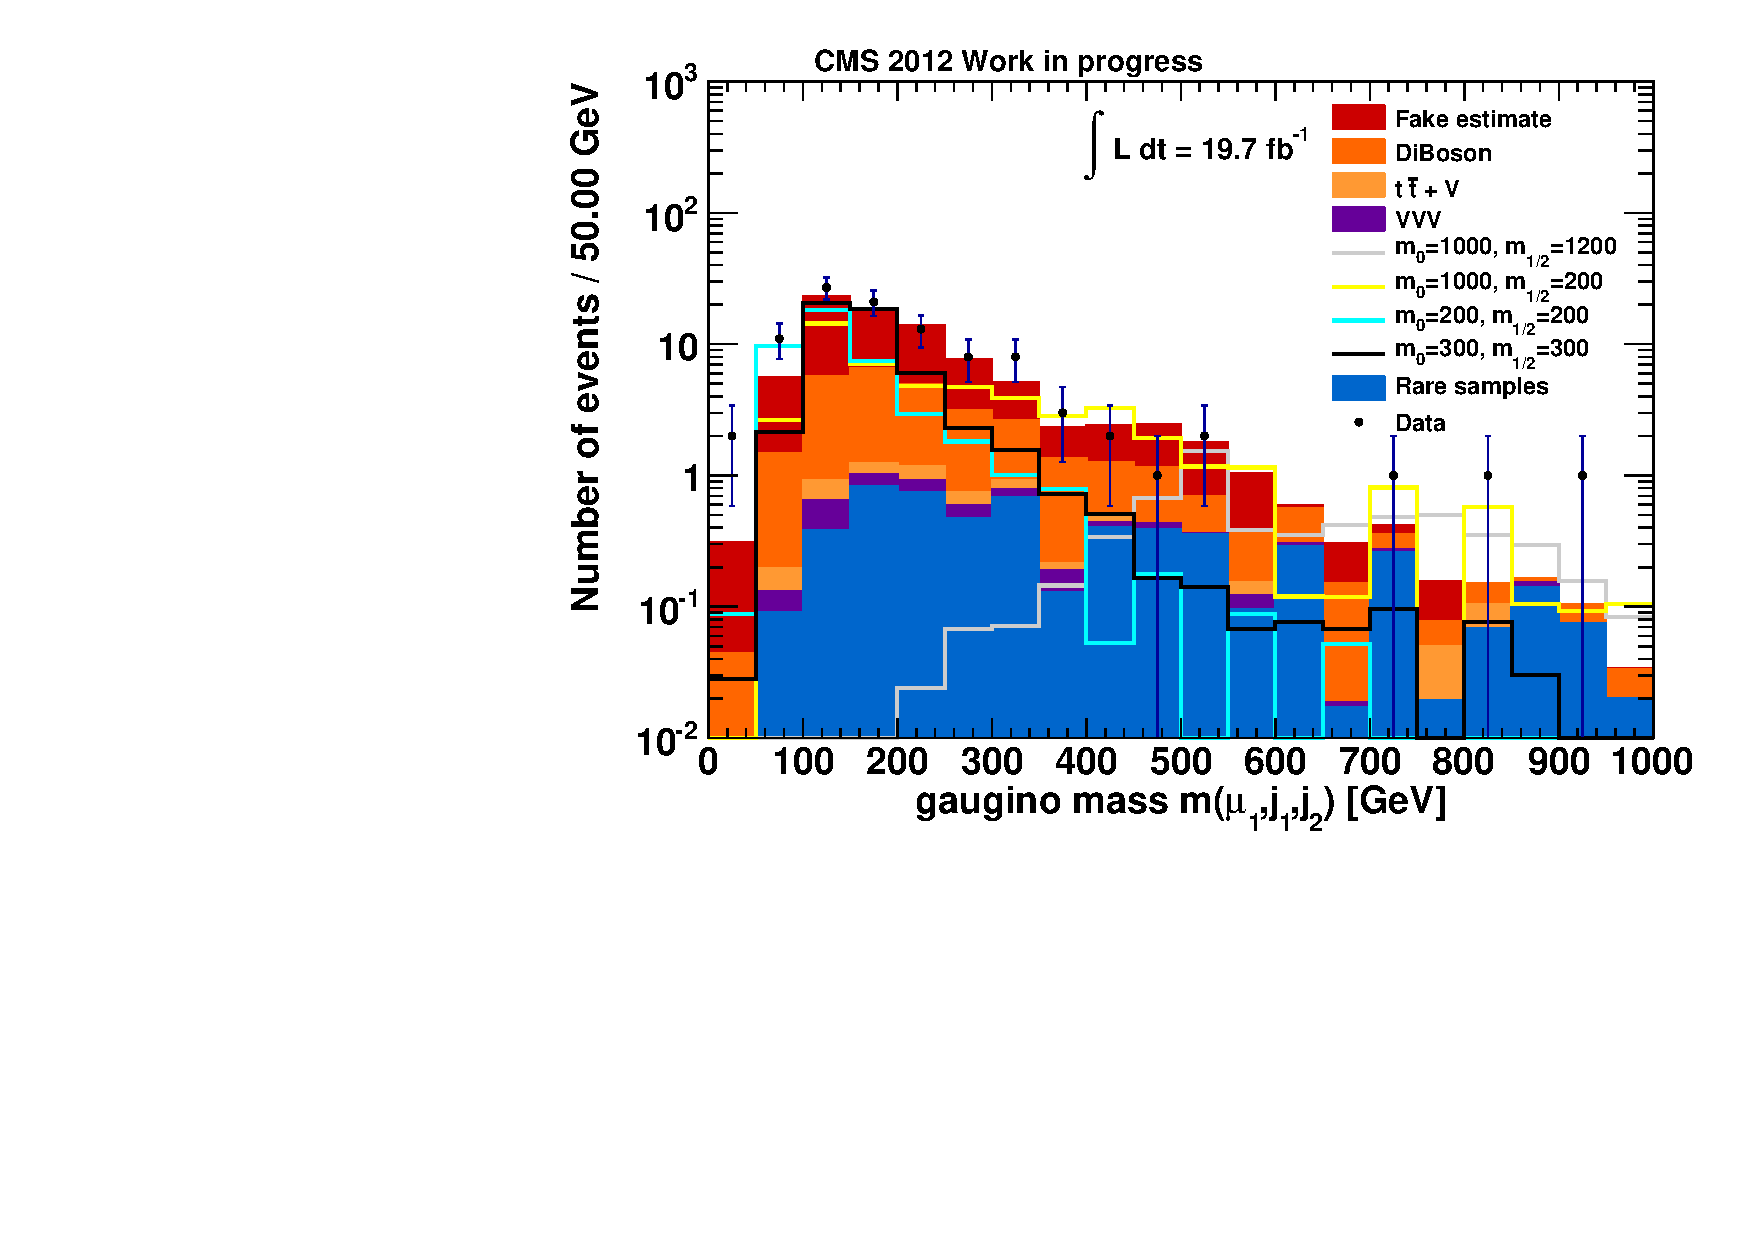
\includegraphics[width=\textwidth]{plots/m_gaugino.pdf}
    \caption{\label{fig:m_gaugino}}
  \end{subfigure}
  \begin{subfigure}[b]{0.495\textwidth}
    \centering
    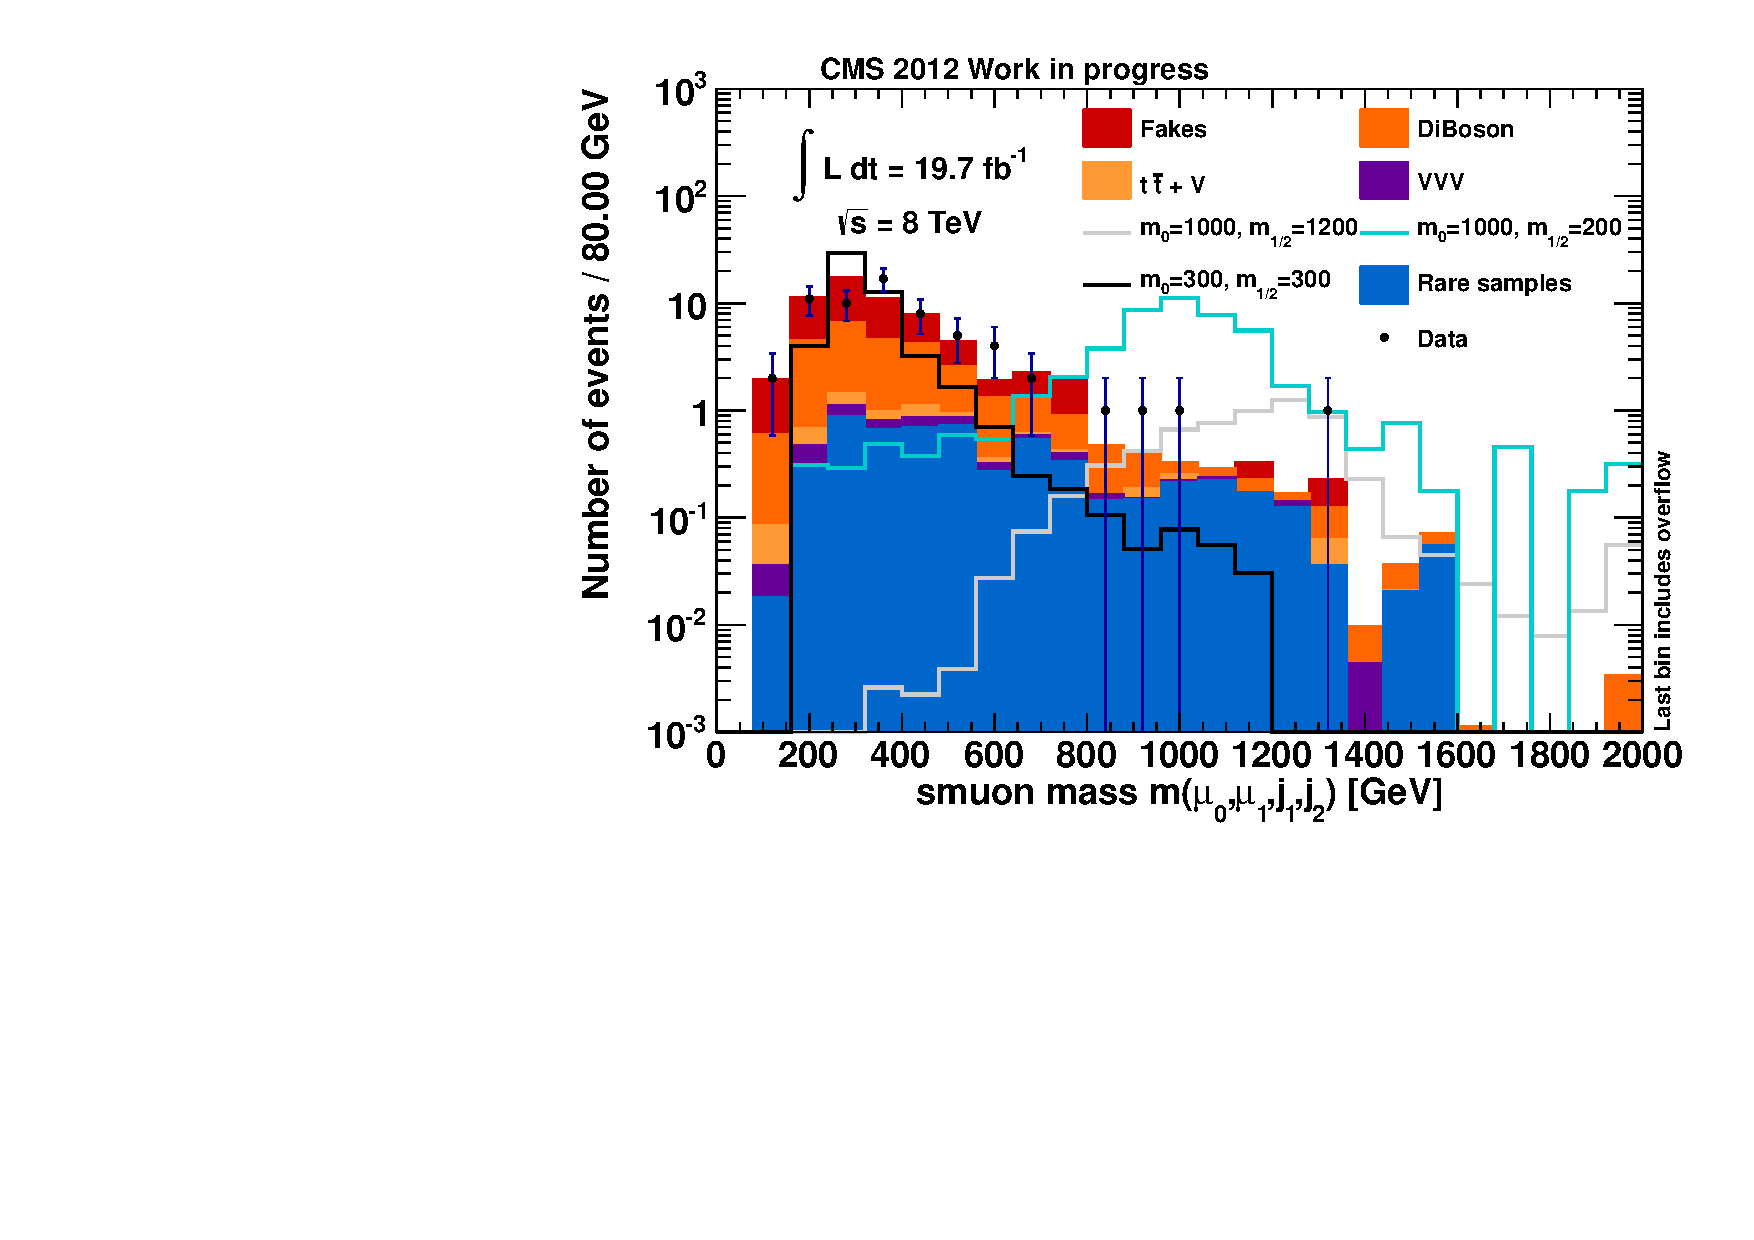
\includegraphics[width=\textwidth]{plots/m_smuon.pdf}
    \caption{\label{fig:m_smuon}}
  \end{subfigure}
  \caption{Mass of the gaugino (\ref{fig:m_gaugino}) and smuon (\ref{fig:m_smuon}). Both are calculated from the invariant masses of the selected two jets and two muons in the smuon case, as well as two jets and the sub leading muon for the gaugino. The distributions include the data-driven background estimate.}
  \label{fig:final-dist}
\end{figure}

Regarding the entire mass region of the final distribution as one bin and summing up the number of events yields table~\ref{tab:nev-msmuon}.

\begin{table}[!htb]
  \centering
  \begin{tabular}{|l|c|c|c|}
    \hline
    \multirow{2}{*}{Backgrounds}    & \multirow{2}{*}{$N_{\text{Events}}$} & \multicolumn{2}{|c|}{Uncertainties} \\ \cline{3-4}
                                    &                                      & stat. & sys.                        \\ \hline \hline
    Fake estimate                   & 54.563                               & 3.170 & 10.913                      \\ \hline
    $W\gamma \rightarrow l\nu 2\mu$ & 1.685                                & 0.460 & 0.855                       \\ 
    $WW \rightarrow 2l 2\nu$        & 0.000                                & 0.000 & 0.000                       \\ 
    $WZ \rightarrow 2l 2q$          & 0.015                                & 0.014 & 0.002                       \\ 
    $WZ \rightarrow 3l \nu$         & 18.465                               & 0.446 & 1.927                       \\ 
    $WZ \rightarrow 2q l \nu$       & 0.029                                & 0.039 & 0.003                       \\ 
    $ZZ \rightarrow 2l 2\nu$        & 0.000                                & 0.000 & 0.000                       \\ 
    $ZZ \rightarrow 2l 2q$          & 0.066                                & 0.029 & 0.007                       \\ 
    $ZZ \rightarrow 4l$             & 2.972                                & 0.047 & 0.294                       \\ \hline
    $t\bar{t} + W$                  & 1.001                                & 0.153 & 0.005                       \\ 
    $t\bar{t} + WW$                 & 0.016                                & 0.002 & 0.001                       \\ 
    $t\bar{t} + Z$                  & 0.294                                & 0.075 & 0.029                       \\ \hline
    $WWW$                           & 0.837                                & 0.078 & 0.080                       \\ 
    $WWZ$                           & 0.197                                & 0.032 & 0.020                       \\ 
    $WZZ$                           & 0.093                                & 0.013 & 0.009                       \\ 
    $ZZZ$                           & 0.006                                & 0.002 & 0.001                       \\ \hline
    $W^- W^-$                       & 1.391                                & 0.159 & 0.706                       \\ 
    $W^+ W^+$                       & 4.046                                & 0.444 & 2.052                       \\ 
    $WW$ Double-parton              & 0.295                                & 0.064 & 0.150                       \\ \hline
    $\sum$                          & 85.972                               & 4.002 & 17.054                      \\ \hline
    Data                            & 101.000                              & -     & -                           \\ \hline
  \end{tabular}
  \caption{Detailed number of events for each background in the distribution of the smuon mass.}
  \label{tab:nev-msmuon}
\end{table}

The statistical uncertainties for the Monte Carlo predictions stem from the generated number of events, which limit the accuracy of the prediction. While the fake estimate has been determined from data, the method itself inherits said statistical uncertainties as background samples are subtracted to determine the tight-to-loose ratio. Respectively adding the uncertainties for every bin of the single- and double-fake estimates in quadrature and propagating them according to equation~\eqref{eq:fakes} yields the statistical uncertainty for this case. All systematic uncertainties are taken from the summary table (Tab.~\ref{tab:sys-uncertainties}). Individual cross section uncertainties are included in accordance to the table's description as well. Overall one can observe an excellent agreement of measurement and simulation. The very slight surplus of data is well within the uncertainties.

Resolving the event count by each background's contribution also reveals the importance of the data-driven background estimate. Combined with the $WZ \rightarrow 3l\nu$ process, they add up to roughly $85\,\pct$ of the entire background prediction.

\section{Calculation of Limits}
\label{sec:calc-of-limits}

As the excess of data is too slight to be considered a discovery, one can translate the result into limits onto two things. The number of events itself and RPV SUSY model parameters. To calculate these, the method commonly used amongst the CMS experiment will be utilized. Details are given in the upcoming section.


\subsection{CLs Method}
\label{sec:cls-method}

To compliment Bayesian and common frequentist methods, the $CL_s$ method~\cite{cls,cls2} has been developed. It is considered a modified frequentist analysis. Compared to the former two, its results are better in cases with low statistics and are less background dependent. The general idea is to compare two hypotheses to a measurement by determining a \textit{confidence level} (\textbf{CL}) for each of them. Confidence levels are defined as the probability of the respective hypothesis describing the measured data.

In regards to high energy particle physics, there are usually two cases to be covered. The null hypotheses being the Standard Model background expectation by itself, while the second hypotheses includes the signal as well. The corresponding likelihoods $\mathcal{L} (x)$ for both cases are the basis of this method. Here, $x$ denotes the background-only scenario for $x = b$ and the background plus signal one for $x = s + b$. The distributions are a function of the cross section corresponding to the relevant processes and therefore effectively also of the number of selected events $n$.

A test statistic $Q$ is used to determine which hypothesis is the better description. It is called the \textit{likelihood-ratio}.

\begin{equation}
  \label{eq:testq}
  Q = \frac{\mathcal{L} (s + b; n)}{\mathcal{L} (b; n)}
\end{equation}

For a result of an experiment, the observed number of events yields a set likelihood-ratio $Q_{\text{obs}}$. The confidence level for either hypothesis to be an accurate description for $Q_{\text{obs}}$, is given as

\begin{equation}
  \label{eq:cl-prob}
  CL_x = P (Q \leq Q_{obs}).
\end{equation}

\noindent Here, $P$ denotes the probability for a test statistic $Q$ being less or equal to the observed statistic $Q_{\text{obs}}$. It is determined through integration.

\begin{equation}
  \label{eq:clx}
  CL_x = \int^{Q_{\text{obs}}}_{-\infty} \frac{d f_x(Q)}{d Q} \text{d} Q
\end{equation}

\noindent The probability distribution functions are denoted by $f_x(Q)$ and are usually determined through pseudo-experiments. For a very well understood background hypothesis, a confidence level in the null hypothesis of $CL_b (Q_{\text{obs}}) \approx 1$ is necessary to claim a discovery. The specific thresholds that $1 - CL_b (Q_{\text{obs}})$ has to fall below, are derived from the Gaussian distribution. This means $2.7 \cdot 10^{-3}$ corresponds to $3\,\sigma$, which is considered ``evidence'', and $5.7 \cdot 10^{-5}$ corresponding to $5\,\sigma$, a discovery.

Excluding the signal (plus background) hypothesis uses the eponymous $CL_s$ quantity instead of $CL_{s+b}$. It is defined as a ratio:

\begin{equation}
  \label{eq:cls}
  CL_s = \frac{CL_{s+b}}{CL_b}.
\end{equation}

\noindent While $CL_{s+b}$ may lead to unphysical results in certain cases, $CL_s$ does not. A prime example is a signal hypothesis that is dominated by its background. Slight fluctuations towards lower values of the latter would lead to a very low $CL_{s+b}$, yielding a strong exclusion limit. As $CL_s$ is not a confidence limit, but a ratio of those, fluctuations like these cancel themselves out.

A signal can be excluded to a confidence level $CL$, when the following relation is fulfilled.

\begin{equation}
  \label{eq:cl-excl}
  1 - CL_s \leq CL
\end{equation}

\section{Modifications}
\label{sec:mods}

Following the recommendations by the CMS and ATLAS collaborations~\cite{clsmod}, a modified test statistic is employed for the $CL_s$ method. To scale the signal strength a parameter $\mu$ is introduced to the formula. It is used to in- or decrease the cross section of the signal prediction while the branching ratios remain constant. Additionally, both the signal and background simulation are subject to a number of uncertainties. To account for those in the limit calculation, a nuisance parameter $\theta$ is introduced.

\begin{equation}
  \label{eq:q-mod}
  Q = - 2 \ln{ \frac{\mathcal{L} (\mu s + b; n, \hat{\theta)}_\mu }{\mathcal{L} (\hat{\mu} \cdot s + b; n, \hat{\theta} )} } \quad \text{ with } \quad 0 \leq \hat{\mu} \leq \mu
\end{equation}

\noindent Here, the pair of parameters $\hat{\mu}$ and $\hat{\theta}$ are determined at the global maximum of the likelihood. $\hat{\theta}_\mu$ on the other hand denotes the conditional maximum likelihood estimator of $\theta$, which also depends on the choice of $\mu$.

% Using the logarithm with a factor of $-2$ allows the test statistic to converge against $\Delta \chi^2$ for a large number of selected events.

To improve the limits, the signal region is subdivided into multiple individual regions. When combining the results for the individual bins, the respective likelihoods have to be multiplied and the overall value is given by

\begin{equation}
  \label{eq:likelihood-product}
  \mathcal{L} = \prod_i \mathcal{L}_i.
\end{equation}

\noindent This enhances the sensitivity, as the influence of large deviations in a certain region is increased.

\section{Limit Graphs}
\label{sec:limit-graphs}

The actual calculation of limits is performed by the \textsc{HiggsCombine} tool~\cite{clsmod,higgscombine}. It employs the \textsc{RooStats} package~\cite{roostats} which is part of the statistical analysis framework \textsc{ROOT}. In line with all CMS publications, the exclusion ranges are calculated to a $95\,\pct$ confidence level as a lower limit ($CL_s \leq 0.05$). The necessary scaling of the signal strength to reach this CL can be achieved through varying the previously introduced modifier $\mu$.

While the result of the calculation is a limit on the signal cross section $\sigma$, it can be translated into a limit onto the model parameter $\lambda^\prime_{211}$. As the former scales quadratically with the latter, the following formula has to be used.


\begin{equation}
  \label{eq:xs-lambda-scale}
  \sigma \propto \lambda^\prime_{211} \Rightarrow \lambda^\prime_{211} (95\,\pct\:b CL) = \lambda^\prime_{211} \cdot \sqrt{ \frac{\sigma (95\,\pct\: CL)}{\sigma} } 
\end{equation}



\section{Discussion and Thoughts}
\label{sec:discussion}


\section{Candidate Events}
\label{sec:candidate-events}


\section{Conclusion and Outlook}
\label{sec:conclusion}




%%% Local Variables: 
%%% mode: latex
%%% TeX-master: "document"
%%% End: 
